\section{GraphRule}


Der Volcano Optimierer ist für seine Erweiterbarkeit und Anpassungsfähigkeit bekannt. Aus diesem Grund wurde er als Vorbild für Pyro(J) gewählt. Die Join-Reihenfolge wird bei diesen Systemen durch Regelmengen wie das von Pellenkoft bestimmt. Leider sind diese Systeme zwar erweiterbar jedoch verglichen mit anderen state-of-the-art Enumeratoren ineffizient. Ein solcher Enumerator ist beispielsweise \texttt{MinCutConservative}. Dieses Verfahren ist zwar erheblich effizient, jedoch nicht im selben Masse erweiterbar. Um die Vorteile beider Systeme zu vereinen, wurde von \cite{shanbhag2014optimizing} eine neue Regel mit dem Titel GraphRule vorgestellt. Diese Regel ist die einzige Regel der Regelmenge RS-Graph. Die neue Regelmenge ist keine Erweiterung im eigentlichen Sinne. Sie ersetzt die bisherigen Regelmengen.

Im Folgenden werden die Grundlagen der Regel erläutert, ihr vorgehen vorgestellt und die Geschwindigkeitsverbesserungen, die gemessen werden konnten behandelt.

\subsection{Top-Down-Enumeration}

Um mit der neuen Regel GraphRule zu starten muss zuerst auf alternative Ansätze zur kreuzproduktfreien Erzeugung von Plänen eingegangen werden. Es gibt zwei unterschiedliche Ansätze: Top-Down-Join-Enumeration mit Memorizing und Bottom-Up-Join-Enumeration mit Dynamic Programming. Ein Bottom-Up-Enumerator ist DPccp, der von \cite{moerkotte2006analysis} entwickelt wurde. Der Nachteil dieser Enumeratoren ist, dass die generierten Bäume nicht beschnitten werden können, was bei Top-Down-Join-Enumeratoren der Fall ist.

Der von \cite{dehaan2007optimal} entwickelte Algorithmus TDMinCutLazy ist der erste effiziente Top-Down-Join-Enumerator. Der alternativer top-down Algorithmus TDMinCutBranch, der fast an die Geschwindigkeit von DPccp heranreichte, wurde in der Folge von \cite{fender2011new} präsentiert. Im Gegensatz zu TDMinCutLazy, der auch Kreuzprodukte generierte, nutzte TDMinCutBranch eine Graphen-basierte Enumerationsstrategie, die nur valide Pläne erzeugt.  Auf Basis dieses Algorithmus wurde der weiter verbesserte Algorithmus TDMinCutConservative von \cite{fender2012effective} vorgestellt. Der Algorithmus ist leichter zu implementieren und noch schneller als sein Vorgänger. 



\subsubsection{Generische Top-Down-Enumeration}

Die Funktionsweise eines generischen Top-Down-Enumerators lässt sich am einfachsten an einem Codebeispiel nachvollziehen. Hierzu ist die folgende Notation notwendig zu verstehen:

\begin{itemize}
\item $E$: Kanten zwischen Knoten
\item $V$: Knoten eines Baums
\item $G$: Graph von Kanten und Knoten
\item $R$: Relationen, die auch als Knoten dargestellt werden können
\end{itemize}


\begin{figure}[ht]
  \centering
  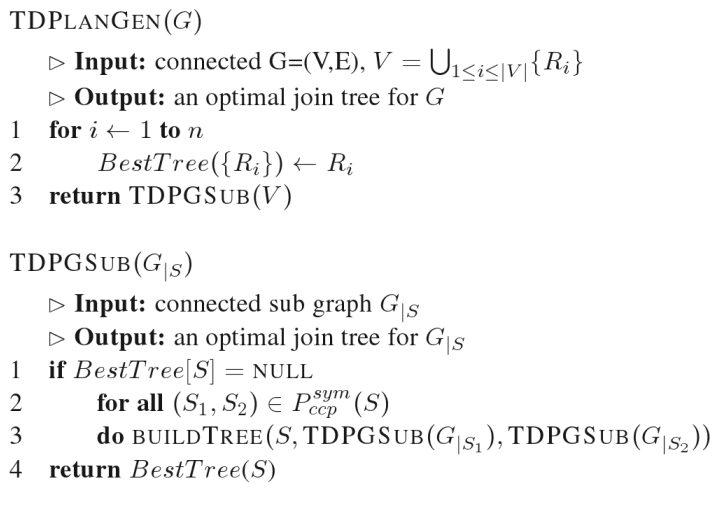
\includegraphics[scale=0.4]{03_Regeln/00_media/TDPlanGen.png}
  \caption{PseudoCode: TDPlanGen}
  \label{TDPlanGen}
\end{figure}


Wie in Abb. \ref{TDPlanGen} zu erkennen, beginnt die Top-Down-Enumeration mit einem Aufruf der Methode \texttt{TDPlanGen(G)} ihr wird ein Graph übergeben. Der Graph besteht aus Knoten und Kanten. Das Ergebnis der Methode ist ein optimaler Join-Tree.

Zuerst wird wie in Zeile 2 zu sehen für jede Relation - sie sind nicht weiter trennbar, daher können keine Alternativen gebildet werden - als beste Variante für ihren jeweiligen Knoten festgelegt. Hierauf wird die Methode \texttt{TDGPSub(V)} aufgerufen. Es wird der gesamte Graph übergeben.


Die Methode \texttt{TDPGSub} prüft zuerst, ob für einen zu untersuchenden Subgraphen bereits ein bester Plan existiert. Ist dies der Fall wird abgebrochen. Falls noch kein bester Plan ermittelt wurde, wir aus dem Subgraphen \texttt{S} durch eine Partitionierungsmethode - sie wird später erläutert - Paare von Subgraphen erzeugt. Aus jedem paar wird ein neuer Baum erstellt. Aus der Menge der neuen Bäume wird dann der beste ausgewählt und ausgegeben. 


\begin{figure}[ht]
  \centering
  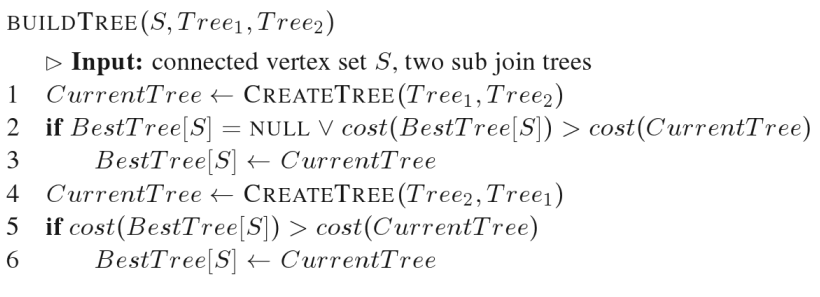
\includegraphics[scale=0.4]{03_Regeln/00_media/BuildTree.png}
  \caption{PseudoCode: BuildTree}
  \label{BuildTree}
\end{figure}

In der Methode \texttt{BuildTree} (vgl. Abb. \ref{BuildTree}) wird aus zweit Teilbäumen zuerst zuerst ein neuer Baum gebildet. Falls die kosten dieses neuen Baums niedriger für den Subgraphen \texttt{S} sind als alle bisher bekannten Pläne, wird der neue Plan als Optimaler Plan gespeichert. Nachdem diese Methode für alle Partitionen eines Subgraphen durchlaufen ist, ist so sichergestellt, dass die Kosten für jeden einzelnen alternativen Graphen verglichen wurden und auch der beste alternative Plan ausgewählt wurde.

\begin{figure}[ht]
  \centering
  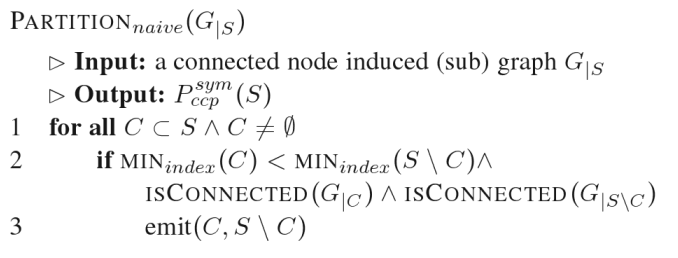
\includegraphics[scale=0.4]{03_Regeln/00_media/Partition.png}
  \caption{PseudoCode: Partition}
  \label{Partition}
\end{figure}


Die Paritionierung eines Graphen in Subgraphen geschieht mit der Methode \texttt{Partition} (vgl. Abb. \ref{Partition}). Aus dem Ausgangsgraphen wird zuerst ein Teilstück \texttt{C} herausgeschnitten. Dieser Teil ist Bestandteil des Subgraphen \texttt{S}. Für jedes TeilStück wird geprüft, ob es mit dem Graphen \texttt{S} verbunden ist. Ist dies der Fall wird ein neues Paar an Subgraphen erstellt. Es besteht aus aus \texttt{C} und  \texttt{S\textbackslash C}. \texttt{S\textbackslash C} und \texttt{C} ergeben so gemeinsam \texttt{S}.


\subsubsection{Partitionierung mit MinCutConservative}

\begin{figure}[ht]
  \centering
  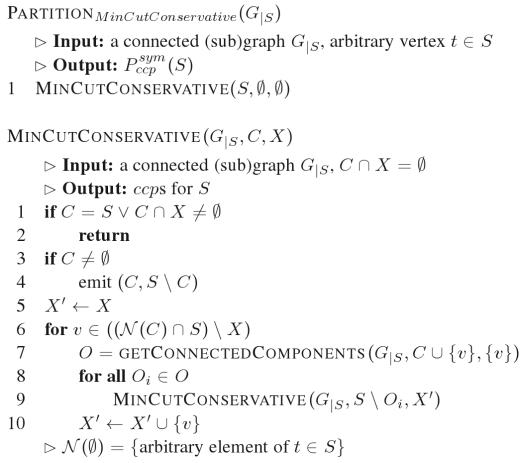
\includegraphics[scale=0.5]{03_Regeln/00_media/MinCutConservative.png}
  \caption{PseudoCode: MinCutConservative}
  \label{MinCutConservative}
\end{figure}

\texttt{MinCutConerservative} ist eine konkrete Implementierung eines Partitionierungsalgorithmus, der auch für GraphRule zum Einsatz kommt. In bestimmten Szearios wie sternförmigen Abfragen, kann die generierung von jeder Teilmenge \texttt{T} eines Subgraphen \texttt{S} exponenziellen Overhead erzeugen, da die meisten komplementären Bäume \texttt{S\textbackslash C} nicht miteinander verbunden sind und somit keine validen, kreuzprduktfreien Teilbäume entstehen. Um zu vermeiden, dass ein komlementärer Baum entsteht, der nicht verbunden ist, wird in diesem konservativen Ansatz nur ein \texttt{C} gewählt, dessen Komplement auch verbunden ist. 







\subsection{Transformationsregel: GraphRule}

Die GraphRule bedient sich der zuvor vorgestellten Implementierung von Top-Down-Enumeratoren. Die Regel, um kompatibel zu anderen Regel und den Regelmengen zu sein, verwendet das selbe Interface wie andere Regeln: \texttt{GraphRule($\Join, E_1, E_2, parent$)}.  Ziel der Regel ist es alle möglichen Transformationen für einen initialen Anfragegraphen mit nur einem Aufruf auszugeben. 

\begin{figure}[ht]
  \centering
  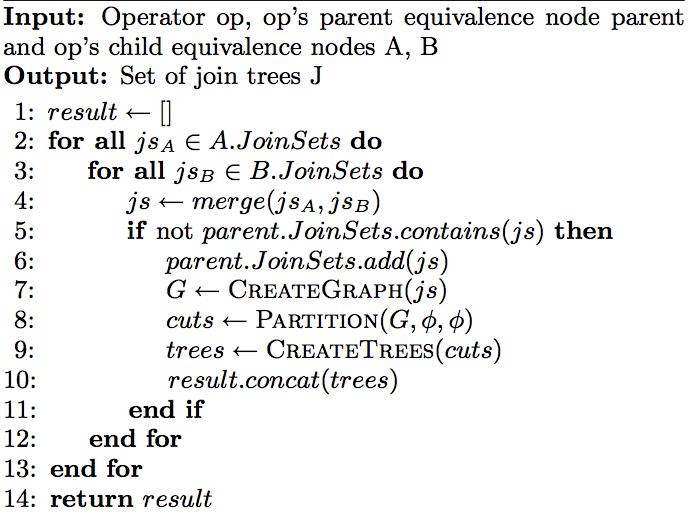
\includegraphics[scale=0.4]{03_Regeln/00_media/GraphRule.png}
  \caption{PseudoCode: GraphRule}
  \label{GraphRule}
\end{figure}

Im Vergleich zu Abb. \ref{TDPlanGen} fällt in Abb. \ref{GraphRule} auf, dass JoinSets verwendet werden. Eine neue \texttt{merge}-Methode verwendet wird und \texttt{CreateGraph} als Methode vorkommen. Ein weiterer grundlegender unterschied ist, dass anstatt von Knoten, die Relationen repräsentieren, Äquivalenzklassen zum Einsatz kommen.





Daher wird der Operator, die linke und rechte Äquivalenzknoten sowie der Vater-Äquivalenzknoten übergeben. Aus der Menge der Join-Sets von linker und rechter Seite wird je ein JoinSet-Element genommen und mit Hilfe einer \texttt{merge}-Operation zusammengefügt. Falls dieses neue Element noch nicht Teil der Menge der JoinSet-Elemente des Vater-Äquivalenzknotens ist, wird weiter fortgefahren und das neue Element dem Vater bekanntgegeben. Aus dem neuen JoinSet-Element wird mit der Methode \texttt{CreateGraph} ein JoinGraph erzeugt. Dieser JoinGraph wird mit einer Partitionierungsmethode getrennt und so einzelne zusammenhängende Stücke des Graphen gebildet, die durch die Methode \texttt{CreateTree} zu einem neuen Baum zusammengefügt werden und damit ein Ergebnis bilden. Sobald über alle Join-Sets der linken und rechten Seite ($E_1, E_2$) iteriert wurde, kann das Gesamtergebnis zurückgeliefert werden. Eine weitere Ausführung der Regel ist ab diesem Moment nicht mehr notwendig, da bereits alle Pläne gefunden wurden.


Im Gegensatz zu den bisher vorgestellten Regeln, sind hier mehrere Routinen Teil der Regel und eine komplexere Bearbeitung notwendig. Die einzelnen Bestandteile \texttt{merge}, \texttt{CreateTree}, \texttt{Partition}, \texttt{CreateGraph} werden nun im Detail angesprochen:


\subsubsection{merge}

Die \texttt{Merge}-Methode hat zwei Input Parameter. Jeder Parameter ist ein JoinSet-Element und kann beispielsweise ein Bitvektor sein. Diese beiden Vektoren werden zusammengefügt, so dass sie eine Repräsentation für beide JoinSet-Elemente bilden. Dieser neue Wert wird zurückgegeben.


\subsubsection{Partition}

%In der Partition Subroutine wird aus einem verbundenen Join-Graphen wird aus der Menge der Knoten, die aus Subsets S_1 und S_2 gebildet werden wobei S_1 und S_2 = S sind. Wenn diese gefunden sind, dann glt dies auch für S_1 und S_2 auch für S_2 und S_1. Da es unterschliedliche Graph Based Partitionierungsalgorithmen gibt, wurde einer ausgewählt das ist MinCutConservative. Es wurde sich für diesen Algorithmus entscheiden, da er der performantestete ist. [Hier 6]





